\documentclass[a4paper]{article}

\usepackage{pgfplots}

\usepgfplotslibrary{statistics}

\begin{document}
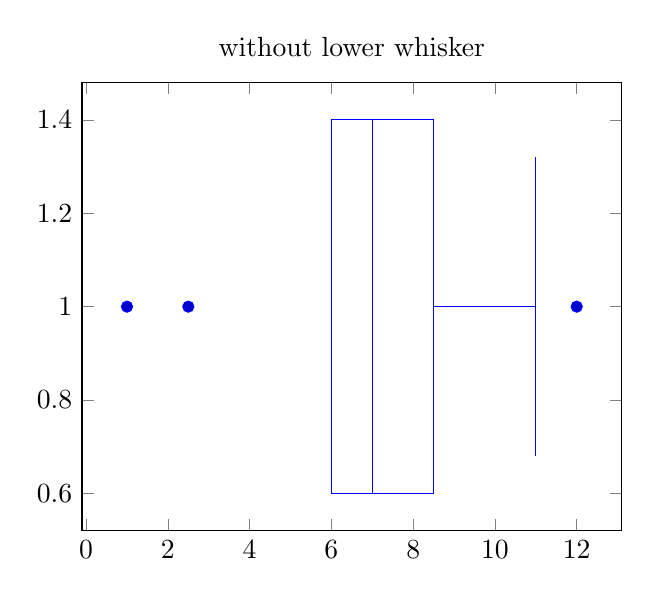
\begin{tikzpicture}
	\begin{axis}[title=without lower whisker,
	]

	\addplot+[
		boxplot prepared={
			lower quartile=6,
			median=7,
			upper quartile=8.5,
			upper whisker=11,
		},
	]
	table[row sep=\\,y=v] {
	v\\
	1\\	2.5\\	12\\
	};

	\end{axis}
\end{tikzpicture}

\begin{tikzpicture}
	\begin{axis}[title=without whiskers]
	\addplot+[
		boxplot prepared={
			lower quartile=6,
			median=7,
			upper quartile=8.5,
		},
	]
	table[row sep=\\,y=v] {
	v\\
	1\\	2.5\\	12\\
	};

	\end{axis}
\end{tikzpicture}

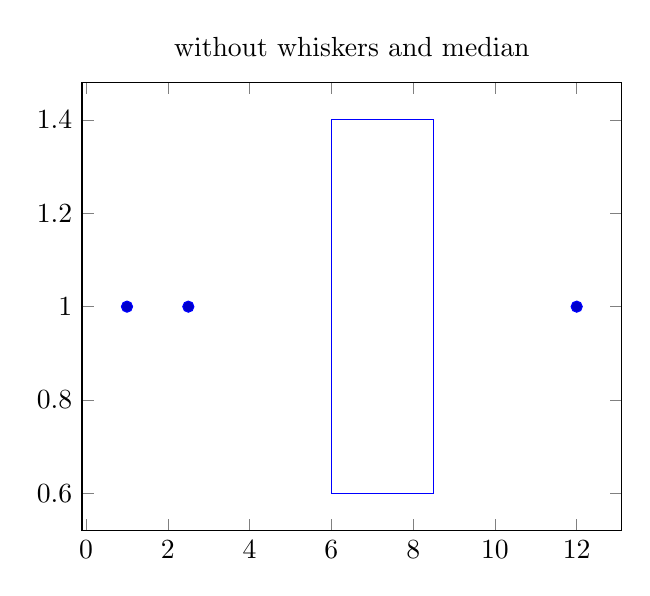
\begin{tikzpicture}
	\begin{axis}[title=without whiskers and median]
	\addplot+[
		boxplot prepared={
			lower quartile=6,
			upper quartile=8.5,
		},
	]
	table[row sep=\\,y=v] {
	v\\
	1\\	2.5\\	12\\
	};

	\end{axis}

\end{tikzpicture}

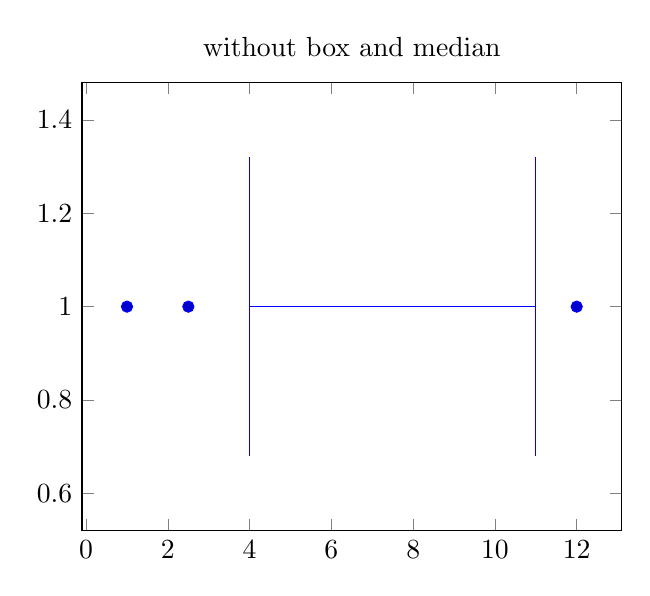
\begin{tikzpicture}
	\begin{axis}[title=without box and median]
	]

	\addplot+[
		boxplot prepared={
			lower whisker=4,
			lower quartile=6,
			upper whisker=11,
		},
	]
	table[row sep=\\,y=v] {
	v\\
	1\\	2.5\\	12\\
	};

	\end{axis}
\end{tikzpicture}
\end{document}

